\section{Method Validation}

  With a defined method and computational setup a varaity of simulations can be run to observe the accuracy and behaviour of the method.
  An examination of a typical simulation will show if the expected behaviour is observed, validating the method as functioning.
  A convergence analysis for the method can be done to confirm that solutions from different grid sizes approach a single solution as they become more precise.
  This convergence test will also show the thresholds for an accurate simulation result, to help reduce the computiation times.
  With a well-established method, the comparison between semi- and fully-implicit methods can be done.

\subsection{Basic Simulations}

  Using Algorithm \ref{alg:iterateCM}, simple scenarios can be tested as a first verification on the method.

  % Too simple/useless visual. Instead maybe have a graph of the standard deviation between gridpoints and show that it stays 0 (or constant?) with time.
  %
  %The most simple test would be homogenous initial conditions, $M = 0.1, C = 1 \forall x \in \Omega$.
  %This test would serve mainly as a confirmation that the method can solve (\ref{equ:model_system}) with the most trivial of initial conditions accurately.
  %The solutions in Figure \ref{fig:basic_homo} show that with homogenous initial conditions, the solution remains homogenous with time.
  %
  %\begin{figure}
  %  \centering
  %  \begin{tabular}{c}
  %  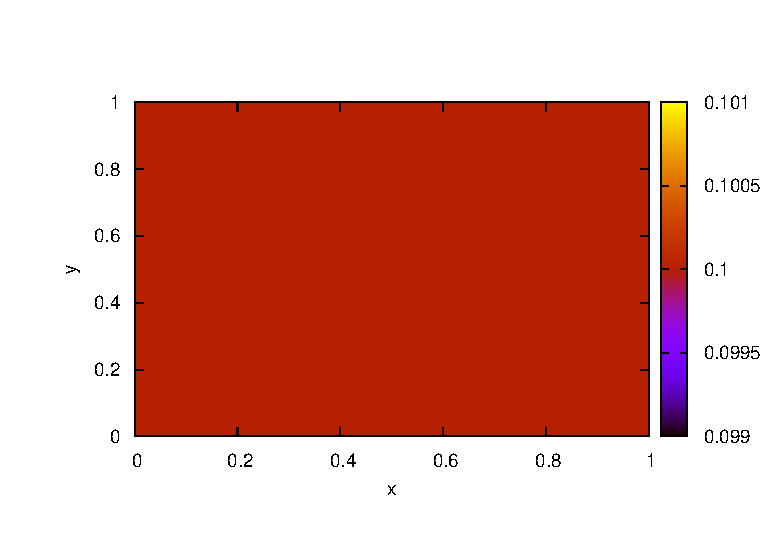
\includegraphics[scale = 0.8]{basic_homo_t0} \\ 
  %  (a) \\
  %  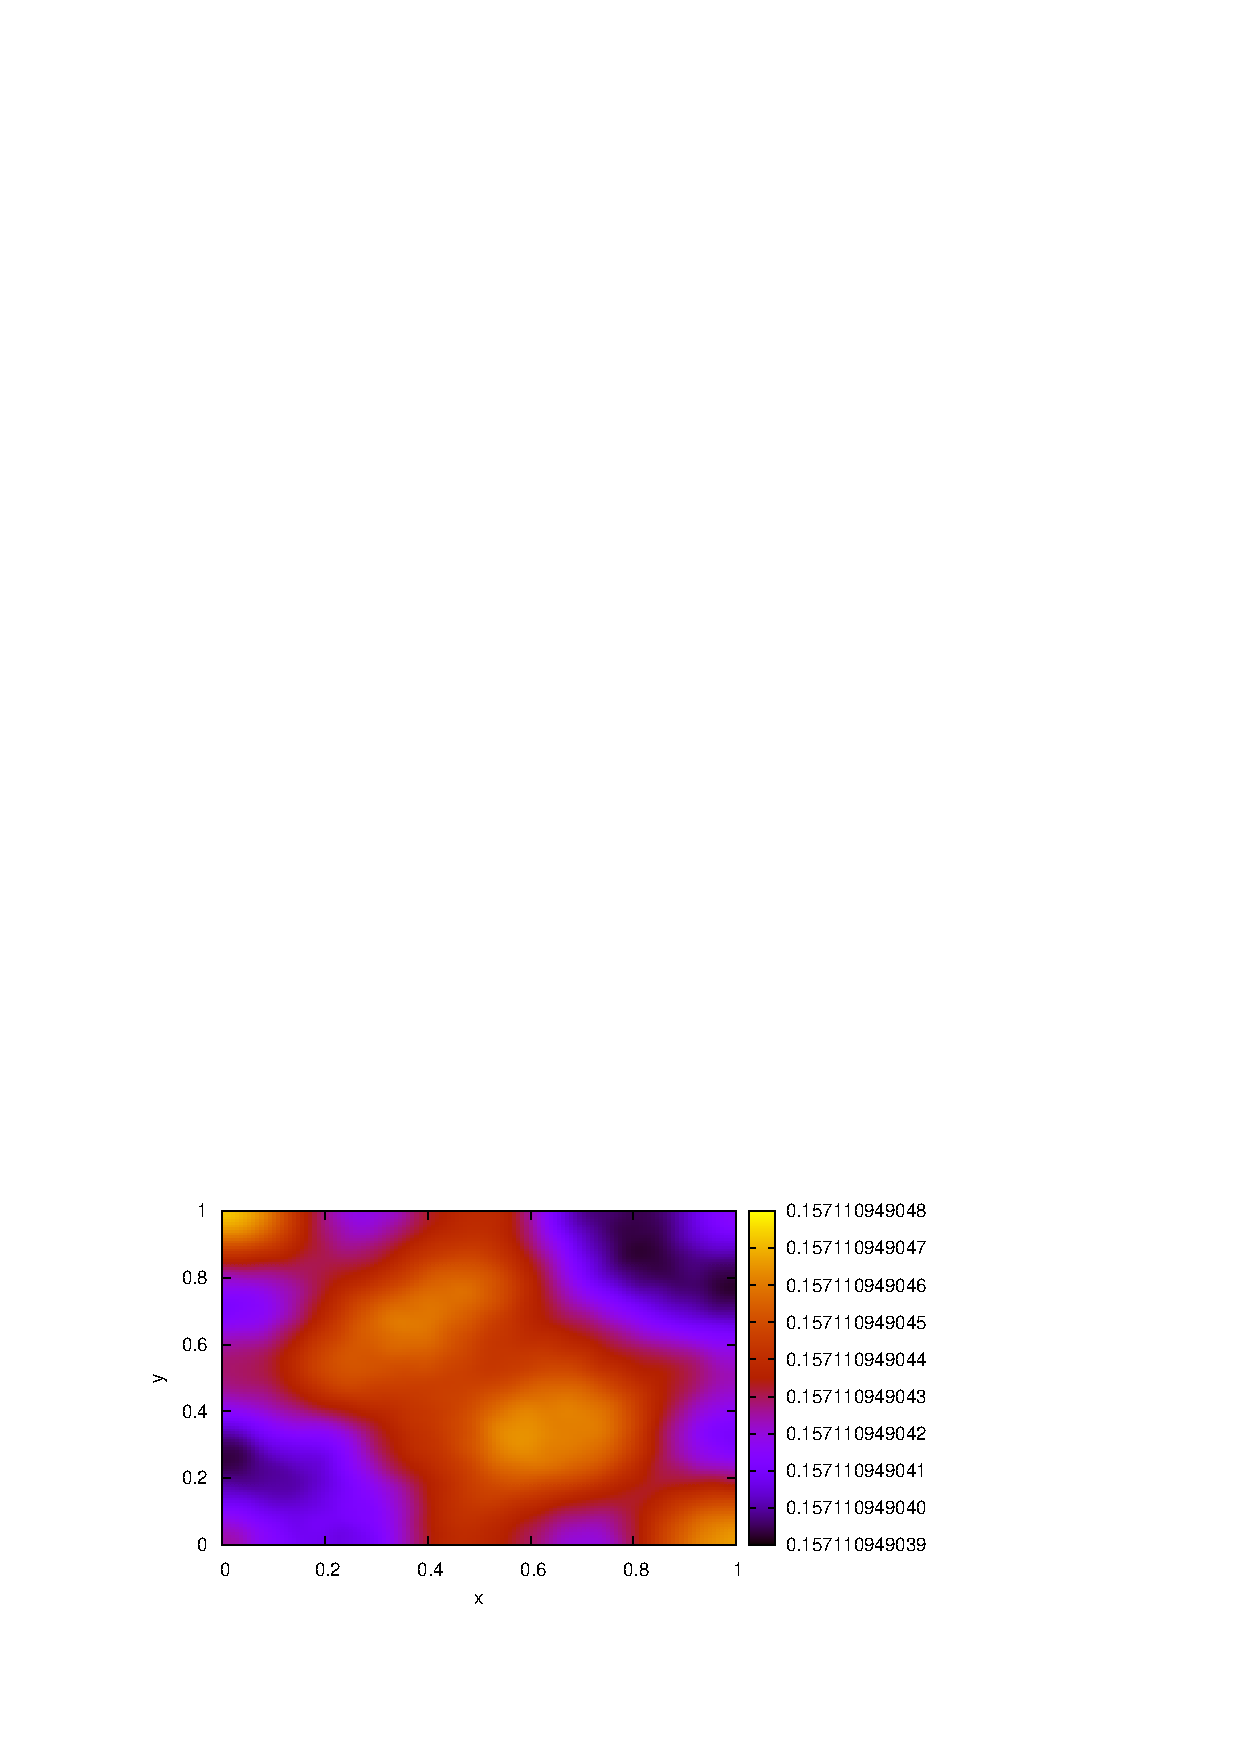
\includegraphics[scale = 0.8]{basic_homo_t10} \\
  %  (b)
  %  \end{tabular}
  %  \caption{Basic homogenous solutions, with $M = 0.1, C = 1 \forall x \in \Omega$. 
  %    The solution stay homogenous with time, as seen by comparing (a) the initial solution at $t = 0$, and (b) at $t = 10$.}
  %  \label{fig:basic_homo}
  %\end{figure}
  

  A simple test would be to check if the spatial discretization can preserve specific characteristics of the solutions.
  One example of this would be seeing if a 1D initial condition could be preserved as time progresses.
  Having all of the biomass on one boundary of $\Omega$, for example across the $y$-axis, would qualify as a 1D intial condition.
  These initial conditions will be defined as:
  \begin{equation} \label{equ:basic_init_trav_wave}
    \begin{aligned}
    M &= \begin{cases}
      -\left( \frac{h}{d^4} \right) x^4 + h & \text{, if } y \le d \\
      0 & \text{, otherwise}
    \end{cases} \\
    C &= 1
    \end{aligned}
  \end{equation}
  where $h = 0.1$ and $d = \frac{5}{128}$.
  Here, $h$ and $d$ represent the height and depth of the innoculation site. 

  The solution shown in Figure \ref{fig:basic_trav} shows that the 1D characteristic of the biomass stays at a later time. 

  \begin{figure}
    \centering
    \begin{tabular}{c c}
      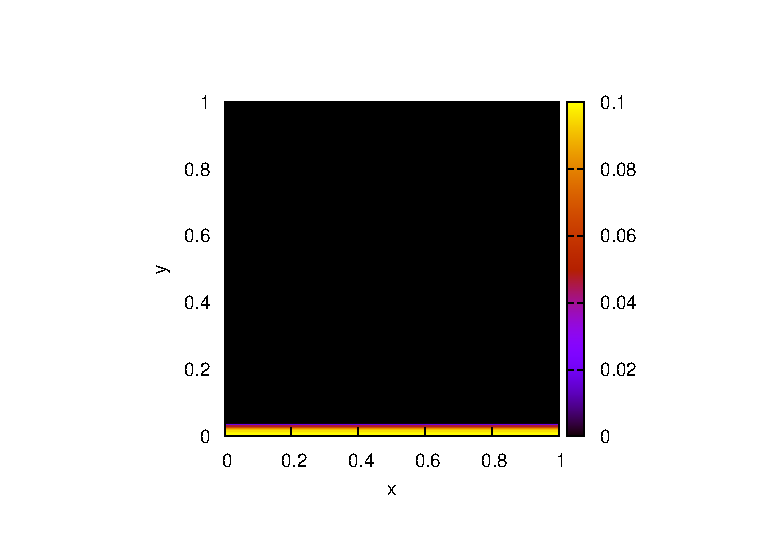
\includegraphics[scale = 0.7]{basic_trav_wave_M_t0} & 
      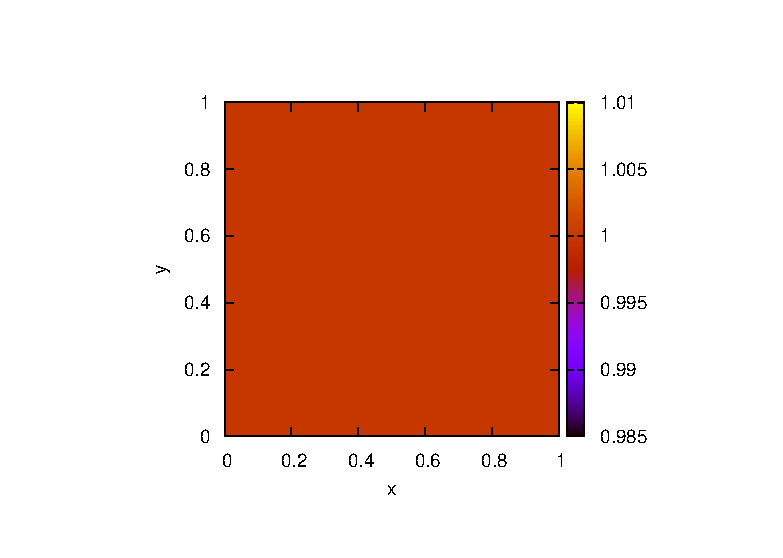
\includegraphics[scale = 0.7]{basic_trav_wave_C_t0} \\
      (a) & (b) \\
      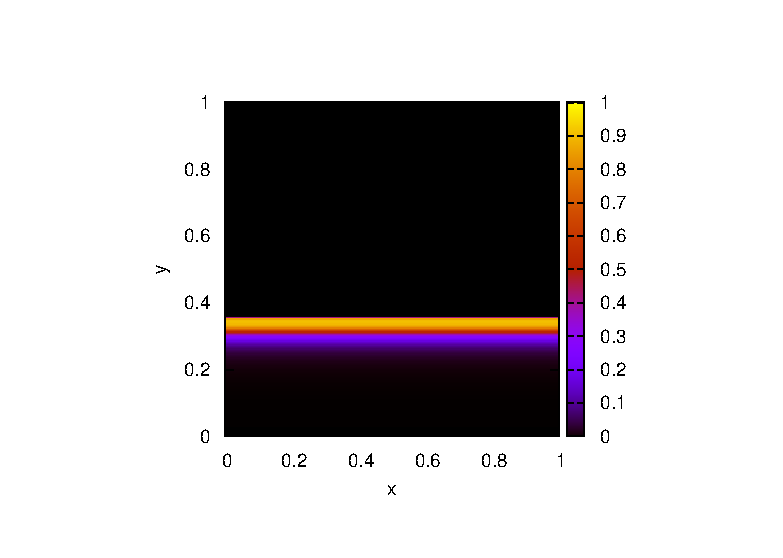
\includegraphics[scale = 0.7]{basic_trav_wave_M_t40} &
      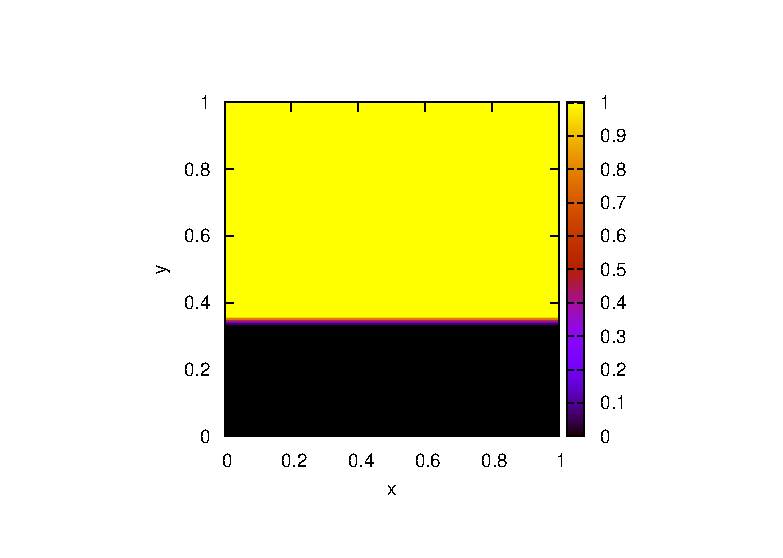
\includegraphics[scale = 0.7]{basic_trav_wave_C_t40}\\
      (c) & (d)
    \end{tabular}
    \caption{Solutions for (ac) $M$ and (bd) $C$ with 1D initial conditions defined in (\ref{equ:basic_init_trav_wave}) at (ab) $t = 0$ and (cd) $t = 40$. Computed with a $1025 \times 1025$ grid and a timestep of $\Delta t = 10^{-3}$.}
    \label{fig:basic_trav}
  \end{figure}

  Another characteristic to observe would be if a spherical initial condition remains spherical.
  Using intial conditions for the biomass,
  \begin{equation} \label{equ:basic_spherical}
    M = \begin{cases}
      - \frac{h}{d^2} \left( x - 0.5)^2 + (y - 0.5)^2 \right) + h  & \text{, if } (x - 0.5)^2 + (y - 0.5)^2 < d^2 \\
      0 & \text{, otherwise}
    \end{cases},
  \end{equation}
  a test can be tried to see if the spherical nature of the solution is kept as time progresses.
  This can be seen in Figure \ref{fig:basic_spherical}, where at different times the shape of the biomass, $M$, is seen to remain spherical.

  \begin{figure}
    \centering
    \begin{tabular}{c c}
      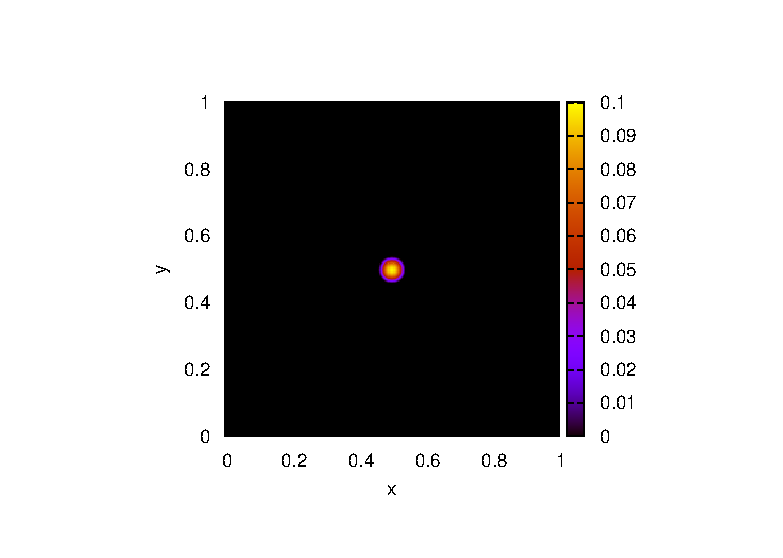
\includegraphics[scale = 0.7]{basic_spherical_M_t0} & 
      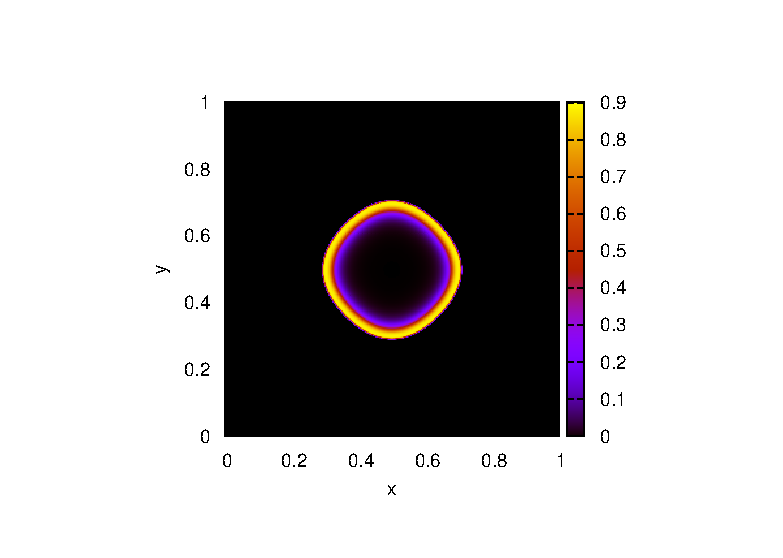
\includegraphics[scale = 0.7]{basic_spherical_M_t40} \\
      (a) & (b)
    \end{tabular}
    \caption{Solutions for $M$ with spherical initial conditions defined by (\ref{equ:basic_spherical}) at (a) $t = 0$ and (b) $t = 40$. Computed with a $1025 \times 1025$ grid and a timestep of $\Delta t = 10^{-3}$.}
    \label{fig:basic_spherical}
  \end{figure}
  
  Both Figure \ref{fig:basic_trav} and Figure \ref{fig:basic_spherical} increase the confidence that the spatial discretization did not introduce any loss of characteristics for the solutions.
    
  %!% Show what happens when it hits the boundary (should mess with total biomass a bit)
  %!% If its bad enough, show that making the grid more refined reduces this (or time step maybe?)
  %!% This shows that the newmann BC doesn't destroy mass (or produce)
  Given the boundary conditions and spatial discretization, there could be a possible source or sink of biomass when it must diffuse along the boundary of the region.
  To ensure this is not the case, the total amount of biomass can be used to compare the simulated amount against the theoretical amount. 
  However, the total biomass cannot be exactly determined with the given growth rate function.
  This means that there will not be anything to measure the validity of the simulation solution against.
  If we let the growth rate be some constant called $a$, the expected total biomass would be of the form $y_0 e^{at}$.
  This can be checked by tracking the total biomass, now called $T_{M}(t)$, with the changed growth rate function, $F(C) = a$.
  The calculation of $T_{M}(t)$ can be done by,
  \begin{equation} \label{equ:total_biomass}
    T_{M}(t) = \int_{\Omega} M(t) dx.
  \end{equation}
  Numerically, this is computed by grid-wise summation,
  \begin{equation}
    T_{M}(t^k) \approx T_{M}^{k} = \frac{ \sum^n_i \sum^m_j M^{k}_{i,j} }{nm}.
  \end{equation}

  %!% If I can figure out how to exactly do this, then add it in....
%  The exact expected biomass can be calculated by computing 
%  \begin{equation}
%    \int_{\Omega} a M(t) dA = M_0 e^{at}
%  \end{equation}
  The simulation setup used will be analogous to that used for Figure \ref{fig:basic_spherical}.
  The one difference will be that the simulation here is ran for a longer time to allow the biomass to diffuse along the boundary, showing the boundary effects.
 
  From Figure \ref{fig:basic_growth} we can see that the total biomass only differs between the computed value and the theoretical value by a relative error less then $0.003$.
  The cases where the error becomes significant are from the region being completely filled with biomass, at which point diffusion is no longer possible.
  The error fluctuates violently here because of this.
  This suggests that the method does not introduce any significant sources or sinks of biomass at the boundary of the region.

  \begin{figure}
    \centering
    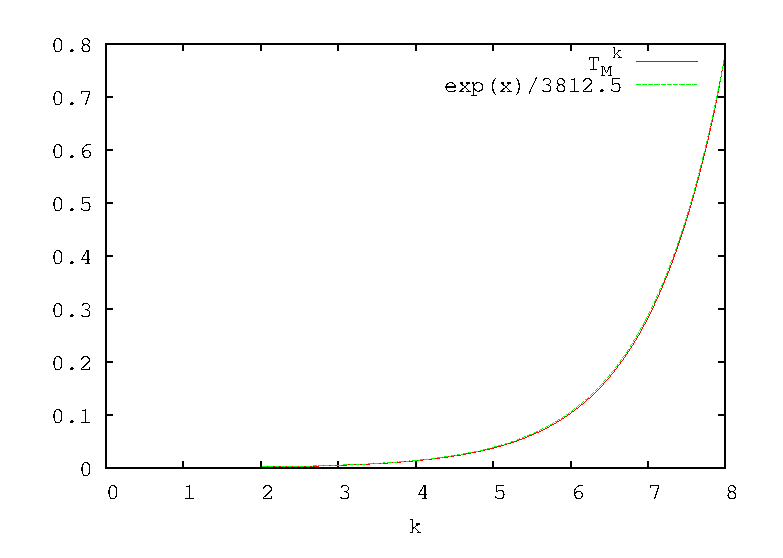
\includegraphics[scale = 0.9]{basic_growth}
    \caption{Plot of the relative error, $\frac{|f_1 - f_2|}{|f_2|}$, between the computed total biomass, $f_1 = T_{M}(t)$, and the theoretical total biomass, $f_2 = y_0 e^x$. 
      The changes after $t = 8$ are from the biomass having completely filled the region $\Omega$.
      This means that there is no physical space for the biomass to occupy and thus the growth slows down to a stop.}
    \label{fig:basic_growth}
  \end{figure}
  
  %!% add mass -conseration between M and C by checking that $M' + \gamma C' = 0$; ie total mass is constant
  %!% Show here the pre-work of integrating over the domain and that the spatial term dissapers and all thats left is the growth terms in both M and C.
  %!% If its interesting, show a graph of M'+gama C vs. t, and try to explain/justify the changes it makes (unless its 0, then just report that its zero and say DATA NOT SHOWN.

\subsection{Convergence Analysis}
  %!%To validate the accuracy of the method, convergence analyses on the spatial and temporal discretizations will need to be made. 
  To validate the accuracy of the method, convergence analyses on the spatial discretizations will need to be made. 
  Then the comparison between the semi- and fully-implicit method established in Algorithm \ref{alg:iterateCM} can investigated.
  First, a metric must be formed to enable consistent comparisons between different simulation solutions. 
  This metric will be referred to as the error. %!% Find a better name fore the norm...

\subsubsection{Error Computations}

  The error is computed by taking the relative normed-difference between two solution in the following fashion:
  \begin{equation} \label{equ:error_comp}
    %!% Maybe at some point try \frac{||u_1 - u_2||}{||u_1|| + ||u_2||}
    \epsilon_{sol} = \frac{||u_1 - u_2||}{||u_2||}
  \end{equation}
  where $u_1$ represents one simulation solution and $u_2$ represents the solution that is theoretically more accurate.
  The theoretical accuracy of $u_2$ derives from the fact that most comparisons will be done between solutions where one is trivially expected to be more precise.
  For our purposes, the solutions we compare will typically vary in only $\Delta x$ or between semi- and fully- implicit.
  These are understood to have the relation that a smaller $\Delta x$, and that the fully-implicit method with the highest tolerance is to be more accurate.
  There is an assumption that both $u_1$ and $u_2$ have the same number of grid points, so that the difference can be taken grid-wise.

  The results of the error computations, named $\epsilon_{sol}$, is a numerical value for the difference between two solutions.
  This depends on the norm used during the computations.
  Here three norms will be used:
  \begin{equation}  \label{equ:norm_l1}
    \ell_1: ||u||_1 = \frac{1}{nm} \sum_{\pi(i,j)}^{nm} |u_{i,j}|
  \end{equation}
  \begin{equation}  \label{equ:norm_l2}
    \ell_2: ||u||_2 = \frac{1}{nm} \sqrt{\sum_{\pi(i,j)}^{nm} (u_{i,j})^2}
  \end{equation}
  \begin{equation}  \label{equ:norm_linf}
    \ell_\infty: ||u||_\infty = \max_{\substack{i=1,\ldots,n \\j=1,\ldots,m}} |u_{i,j}|
  \end{equation}
  These different norms will all be used to create a broader understanding of the error.
  This creates three distinct values for $\epsilon_{sol}$, named $\epsilon_{\ell_1}$, $\epsilon_{\ell_2}$, and $\epsilon_{\ell_\infty}$; each named for the norm used during the computation.
  
 %!% \item What program did I use? (R probably....)
 %!% \item Maybe run though a trivial Fisher equation problem to confirm that it works ?
  % Also mention the Accuracy of the solutions by using the norm of each solution compared to the  most accurate one.... (Maybe take a solution at a higher grid resolution?, not sure what to do here)

\subsubsection{Grid Size Convergence}
%!% Just show the results and state it is slow to converge when F(C) is dependent on C (double check with the older versions of code)
  To observe the validity of the method, a test on the convergence of solutions based on the spatial discritization is done.
  This will involve using the same simulation described in (\ref{equ:basic_init_trav_wave}) due to the simplicity. 
 
  The convergence will be tracked with only two forms of $\epsilon_{sol}$; $\epsilon_1$ and $\epsilon_2$.
  This is because the value of $\epsilon_{\infty}$ doesn't vary with the grid size, since the wave front has a steep interface and tends to lead to inconsistent changes in error.
  Since the use of $\epsilon_{\infty}$ is not a suitable method for measuring the error, the inconsistency does not suggest an invalidity with the method.
  Because of the difference in the number of grid points between different solutions, $u_1$ and $u_2$, only the grid points in the coarser refinement will be used.
  This places a limitation on the selection of grid-sizes since there must be some grid points locations that are the same for two different chosen grid sizes.
  For this purpose, we define the function $s(n) = 2^{n}+1$ for $n \in \mathbb{N}$ to be used as the grid size selection function.
  Now certain grid points will match without the use of linear interpolation.
  Here we do not use the typical grid doubling, $2^n$, because no grid points equal between two different grid size selection, as illustrated in Figure \ref{fig:grid_point_lineup}.

  \begin{figure}
    \centering
    \begin{tabular}{| c | c | c |}
      \hline
      &  $s(n) = 2^{n}+1 $ & $2^n$ \\
      \hline
      $n=2$ 
      & 
      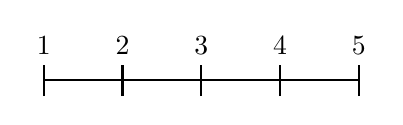
\begin{tikzpicture}
        \draw [thick] (0.0, 1.0) -- (4.0, 1.0);
        \draw [thick] (0.0, 0.8) -- (0.0, 1.2);
        \draw [thick] (1.0, 0.8) -- (1.0, 1.2);
        \draw [thick] (2.0, 0.8) -- (2.0, 1.2);
        \draw [thick] (3.0, 0.8) -- (3.0, 1.2);
        \draw [thick] (4.0, 0.8) -- (4.0, 1.2);

        \node [above] at (0.0, 1.2) {1};
        \node [above] at (1.0, 1.2) {2};
        \node [above] at (2.0, 1.2) {3};
        \node [above] at (3.0, 1.2) {4};
        \node [above] at (4.0, 1.2) {5};
      \end{tikzpicture} 
      &
      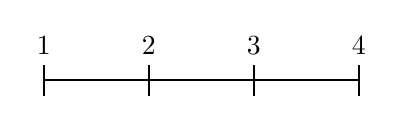
\begin{tikzpicture}
        \draw [thick] (0,1) -- (4,1);
        \draw [thick] (0.0, 0.8) -- (0.0, 1.2);
        \draw [thick] (1.333, 0.8) -- (1.333, 1.2);
        \draw [thick] (2.667, 0.8) -- (2.667, 1.2);
        \draw [thick] (4.0, 0.8) -- (4.0, 1.2);

        \node [above] at (0.0, 1.2) {1};
        \node [above] at (1.333, 1.2) {2};
        \node [above] at (2.667, 1.2) {3};
        \node [above] at (4.0, 1.2) {4};
      \end{tikzpicture}
      \\
      \hline
      $ n = 3 $
      &
      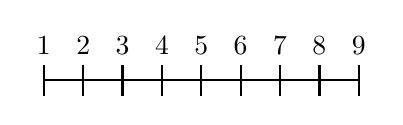
\begin{tikzpicture}
        \draw [thick] (0,1) -- (4,1);
        \draw [thick] (0.0, 0.8) -- (0.0, 1.2);
        \draw [thick] (0.5, 0.8) -- (0.5, 1.2);
        \draw [thick] (1.0, 0.8) -- (1.0, 1.2);
        \draw [thick] (1.5, 0.8) -- (1.5, 1.2);
        \draw [thick] (2.0, 0.8) -- (2.0, 1.2);
        \draw [thick] (2.5, 0.8) -- (2.5, 1.2);
        \draw [thick] (3.0, 0.8) -- (3.0, 1.2);
        \draw [thick] (3.5, 0.8) -- (3.5, 1.2);
        \draw [thick] (4.0, 0.8) -- (4.0, 1.2);

        \node [above] at (0.0, 1.2) {1};
        \node [above] at (0.5, 1.2) {2};
        \node [above] at (1.0, 1.2) {3};
        \node [above] at (1.5, 1.2) {4};
        \node [above] at (2.0, 1.2) {5};
        \node [above] at (2.5, 1.2) {6};
        \node [above] at (3.0, 1.2) {7};
        \node [above] at (3.5, 1.2) {8};
        \node [above] at (4.0, 1.2) {9};
      \end{tikzpicture}
      &
      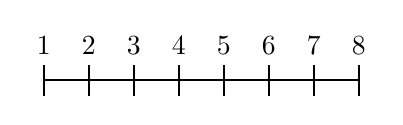
\begin{tikzpicture}
        \draw [thick] (0,1) -- (4,1);
        \draw [thick] (0.000, 0.8) -- (0.000, 1.2);
        \draw [thick] (0.571, 0.8) -- (0.571, 1.2);
        \draw [thick] (1.143, 0.8) -- (1.143, 1.2);
        \draw [thick] (1.714, 0.8) -- (1.714, 1.2);
        \draw [thick] (2.286, 0.8) -- (2.286, 1.2);
        \draw [thick] (2.857, 0.8) -- (2.857, 1.2);
        \draw [thick] (3.429, 0.8) -- (3.429, 1.2);
        \draw [thick] (4.000, 0.8) -- (4.000, 1.2);

        \node [above] at (0.000, 1.2) {1}; 
        \node [above] at (0.571, 1.2) {2};
        \node [above] at (1.143, 1.2) {3};
        \node [above] at (1.714, 1.2) {4};
        \node [above] at (2.286, 1.2) {5};
        \node [above] at (2.857, 1.2) {6};
        \node [above] at (3.429, 1.2) {7};
        \node [above] at (4.000, 1.2) {8};

      \end{tikzpicture}
      \\
      \hline
    \end{tabular}
    \caption{Visualization in 1D to illustrate the choice of $s(n) = 2^{n} + 1 $ instead of $2^{n}$ for the grid size selection.
      Here is can be seen that successive grid size selections using $s(n)$ line up on certain grid points and when using $2^n$ no grid points are equivalent.}
    \label{fig:grid_point_lineup}
  \end{figure}

  
  %!% Makes this use log graph and maybe its a stragith line.
  %!% Also have graphs of how the quatilites of interest change with grid-size (and with t?)
  %!% Maybe have a 2D plot of x = \delta x, y = \delta t, z = \epsilon. showing how it (should) decrease with \delta x and \t.
  %     to the above graph, can later add computation time to it to justify the choice in \delta t and \delta x for the later simulations

  Using the same simulation setup as was done in Figure (\ref{fig:basic_trav}), solutions resulting from different grid sizes based on $s(n)$ are computed for $n = 5, 6, \ldots, 12$.
  In this case, when calculating $\epsilon_{sol} = \frac{| u_1 - u_2 |}{|u_2|}$, we let $u_1$ be the grid size under investigation and $u_2$ be the solutions of the most refined gridsize, $n = 12$.
  This results in a series of values that, if the solutions converge with smaller grid sizes, should have less change.



  \begin{figure}
    \centering
    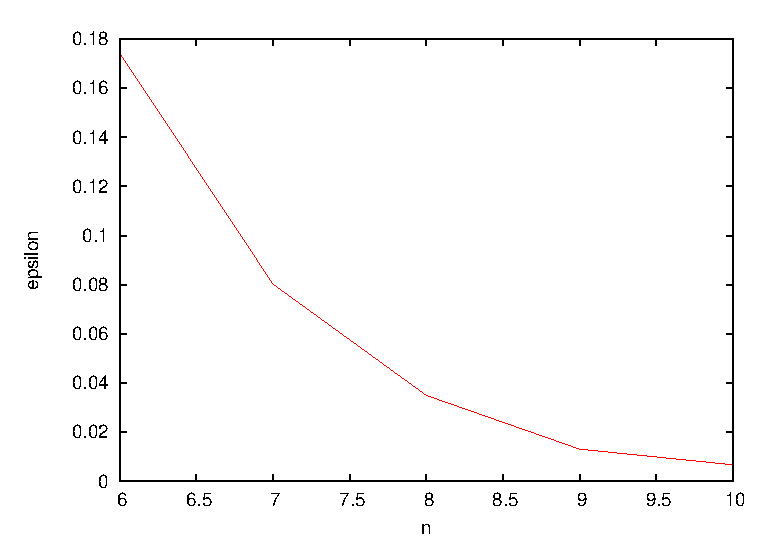
\includegraphics{converge_spatial}
    \caption{Plot showing the convergence of solutions based on changes in $\Delta x$. The computions are of $\epsilon_{\ell_1}$ and $\epsilon_{\ell_2}$ with grid-size following $s(n) = 2^{n}+1$.}
    \label{fig:converge_spatial}
  \end{figure}

  The results from Figure \ref{fig:converge_spatial} show that the solutions converge as the grid size become refined with the grid size.

%!% Also, check the results with a larger and smaller $\Delta t$ to see if they change.

%\subsubsection{$\Delta t$ Convergence}
%
%  A similar convergence analysis will also be performed for the temporal discritizations.
%  This is simply to confirm that the selection of $\Delta t$ is optimal for computation time and for accuracy.
%  The 
%
%  \begin{figure}
%    \centering
%    \begin{tabular}{c c}
%%    \includegraphics{converge_temporal_a.eps} &
%%    \includegraphics{converge_temporal_a.eps} \\
%    (a) & (b) \\
%%    \includegraphics{converge_temporal_a.eps} &
%%    \includegraphics{converge_temporal_a.eps} \\
%    (c) & (d)
%    \end{tabular}
%    \caption{A series of plots showing the convergece of solutions based on changes in $\Delta t$ using $eSoln = 10^n$ for (a) $n = -1$, (b) $n = -4$, (c) $n = -8$, and (d) $n = -12$.} 
%
%  \end{figure}
 
%\subsection{Table of Results}
%
%That list, compute time, "error", number of iterations of linear solver, and number of iterations for ALgorithm 1 for a series of $\epsilon_{sol}$.
%Do this table for a larger $\Delta t$ to see if the algorithm allows for a faster computation with the larger timesteps.
%
%Be extrodinaryly pedantic on everything here.
%Try for something like a paragraph for each item in the table; explain how it's computed, why we pick this measure, what we expect, and what it will say about the results....
%


